\documentclass[12pt]{article}
\usepackage{graphicx}
\usepackage{amsmath}
\usepackage{tikz}
\title{C-Space of a 2-link Planar Manipulator Arm}
\date{}
\begin{document}
\maketitle
\section*{Introduction}
In robotic motion planning, the workspace is the physical environment containing the robot and obstacles, while the configuration space (C-space) represents all possible joint configurations. Each point in C-space corresponds to a unique robot pose, and the mapping from workspace to C-space becomes highly non-linear when obstacles are present. We begin by exploring a discretized angle-based method that generates binary collision maps for various obstacle positions. To overcome the limitations of this approach, we later adopt a geometric method that starts by identifying safe angular ranges for the first link of a 2R manipulator, and then extends to the second link for interpretable collision avoidance.

\section{Binary Matrices Approach}
In this method, we start with a simple 2R planar manipulator, which is kept near a small rectangular obstacle. The goal of this process is to find the set of joint angles of the robot, for which there is a collision-free motion. We are tasked with mapping the C-Space from the given workspace. For this, we use MATLAB R2024b. We start off by discretizing the values of both the joint angles, in steps of 2 degrees. Let us denote first joint angle as $\theta_1$, and the second joint angle measured with respect to the first link, as $\theta_2$. So now, we have both these angles taking values such as 0, 2, 4, ....upto 360 degrees. We assume there are no joint limits for this analysis.
\newline
We can observe that each unique configuration of the robot needs 2 parameters, which are basically $\theta_1$ and $\theta_2$. Since we discretize in steps of 2 degrees, both $\theta_1$ and $\theta_2$ can take 181 different angle values, starting from 0 and going till 360 degrees. So there are 181 x 181 unique configurations of the robot that is possible for the chosen discretization. We put all of these 181 x 181 values inside a square matrix having 181 rows and 181 columns. Also, there will be some configurations of the robot which will collide with the obstacle, while others may not. For all the configurations that collide with some part of the obstacle, we assign a value of 1 in the corresponding position of the 181 x 181 matrix. Collision free positions are denoted by 0 in the matrix. Now we finally have a matrix that contains only zeros and ones. We call this the binary matrix which tells us which configurations are collision free, and those which are collision prone.
\newline
We shall now get a visual idea of the C-Space by plotting the binary matrix. Create a plot with X-Axis as $\theta_1$ and Y-Axis as $\theta_2$. Use the binary matrix values to construct the plot. The collision prone configurations of the robot will be denoted by the number 1 in the matrix; so while plotting these, we assign black colour. Collision free configurations need not be plotted explicitly in any colour, as we are already plotting the collision prone positions in black. After plotting completely, we can get a plot which is shaded black in some regions, and others regions are just plain. The black regions correspond to all the collision-prone configurations, while the plain regions are collision-free configurations.
\begin{figure}[h]
    \centering
    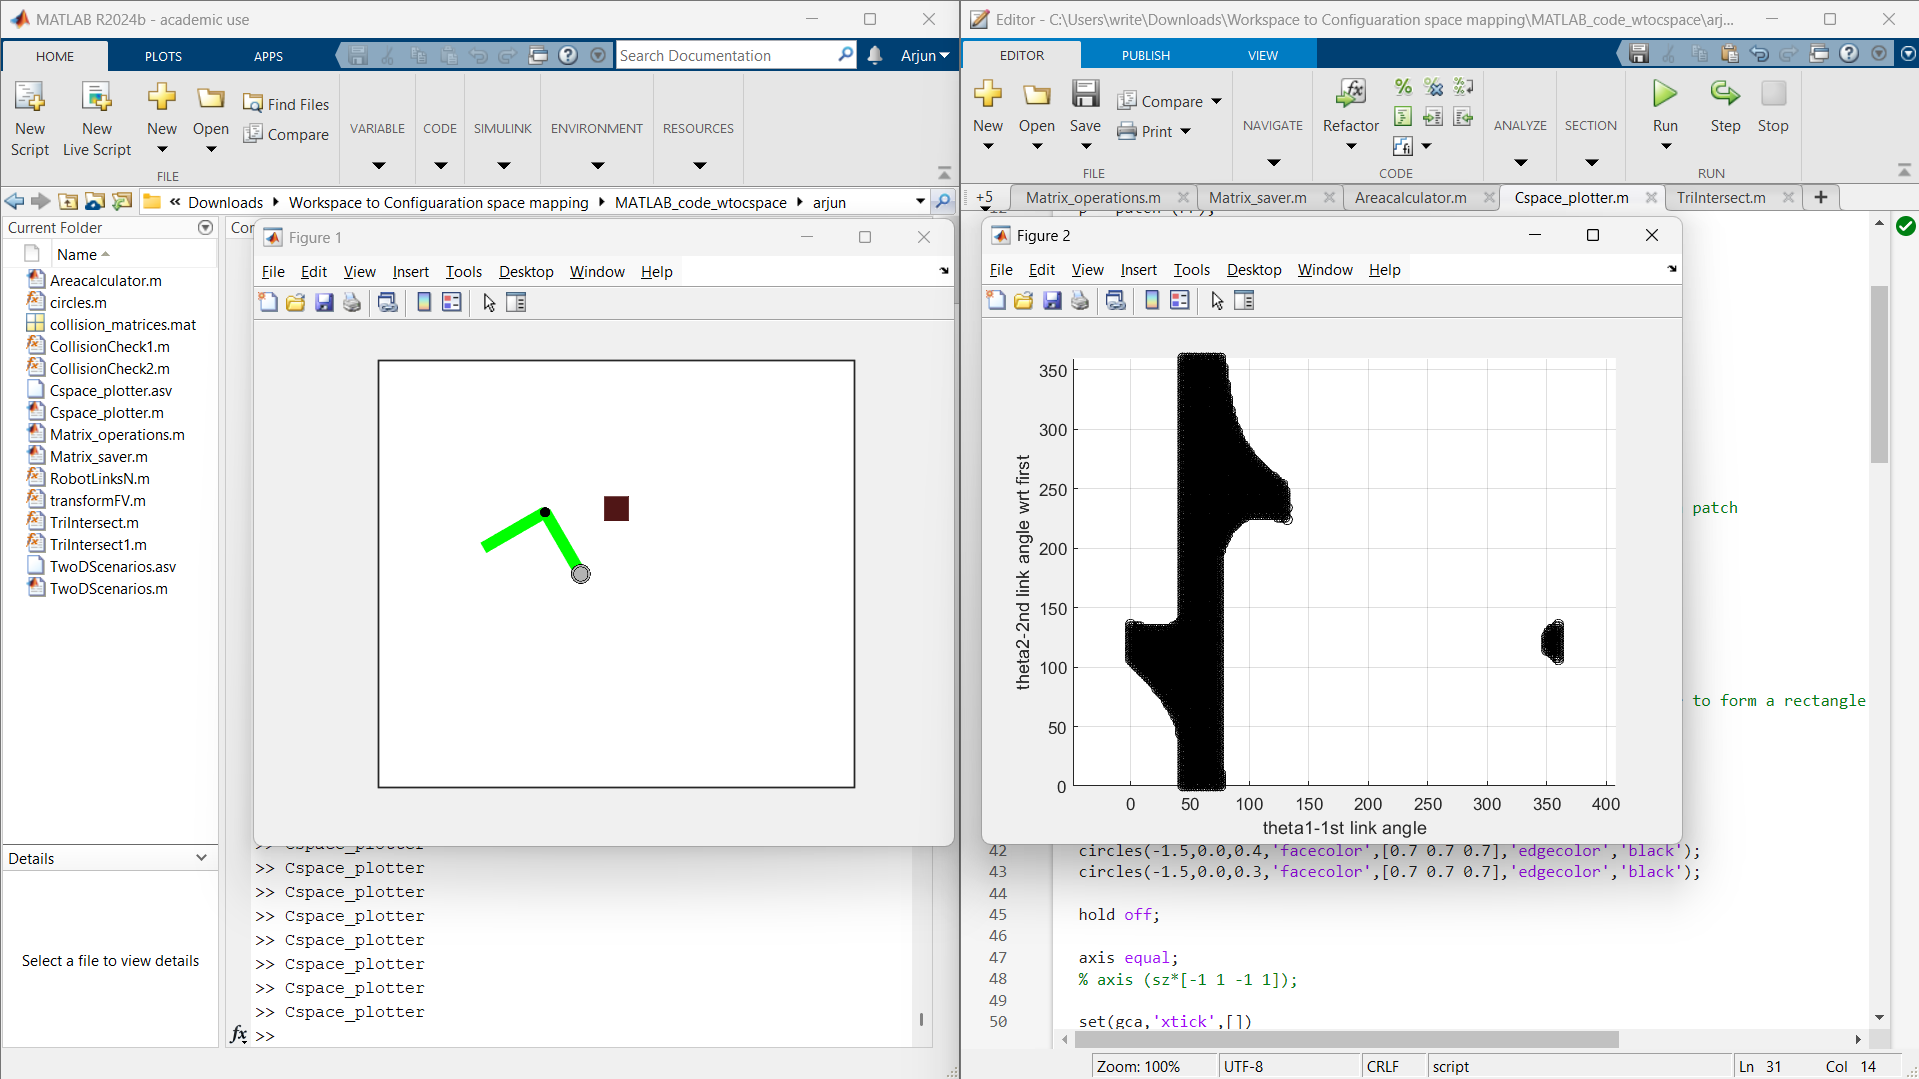
\includegraphics[width=1.0\textwidth]{Screenshot 2025-05-15 115430}
    \caption{Window on the right shows the plot between $\theta_2$ and $\theta_1$}
    \label{fig:1}
\end{figure}
\newline
Next, we try to observe the variation in the C-Space plot, for a given input motion of the obstacle. We start off by considering a simple unidirectional translation of the obstacle along the vertical direction; and we plot the C-Space by sampling different positions that the obstacle would have visited during its motion. We keep incrementing the Y-coordinate of the obstacle center in steps of 0.25 units, upto 5 units. So we get - 
\[
\frac{5}{0.25} + 1 = 21 \text{(considering initial position also)}
\]
So now we have 21 different positions of the obstacle, and we will have a 181 x 181 binary matrix for each of these positions. So in total, we have 21 different binary matrices. We now create an animation with these 21 different plots, where we can visualize how to C-Space is changing when the obstacle moves vertically in a straight line. Following figures show how the C-Space is changing for the unidirectional motion of obstale.
\begin{figure}[h]
    \centering

    \begin{minipage}{0.48\textwidth}
        \centering
        \includegraphics[width=\linewidth]{C-Space_series/1.png}
    \end{minipage}
    \hfill
    \begin{minipage}{0.48\textwidth}
        \centering
        \includegraphics[width=\linewidth]{C-Space_series/2.png}
    \end{minipage}

\end{figure}
\clearpage  % forces a page break

\begin{figure}[h]
    \centering

    % Row 2
    \begin{minipage}{0.48\textwidth}
        \centering
        \includegraphics[width=\linewidth]{C-Space_series/3.png}
    \end{minipage}
    \hfill
    \begin{minipage}{0.48\textwidth}
        \centering
        \includegraphics[width=\linewidth]{C-Space_series/4.png}
    \end{minipage}

    \vspace{0.5cm}

    % Row 3
    \begin{minipage}{0.48\textwidth}
        \centering
        \includegraphics[width=\linewidth]{C-Space_series/5.png}
    \end{minipage}
    \hfill
    \begin{minipage}{0.48\textwidth}
        \centering
        \includegraphics[width=\linewidth]{C-Space_series/6.png}
    \end{minipage}

    \vspace{0.5cm}

    % Row 4
    \begin{minipage}{0.48\textwidth}
        \centering
        \includegraphics[width=\linewidth]{C-Space_series/7.png}
    \end{minipage}
    \hfill
    \begin{minipage}{0.48\textwidth}
        \centering
        \includegraphics[width=\linewidth]{C-Space_series/8.png}
    \end{minipage}
\end{figure}\clearpage
We can observe that until the obstacle is within the circle described by the first link, the C-Space plot is a continuous layer without any break (first 6 figures above show this). Once the obstacle is outside the circle described by the first link, the C-Space becomes a discontinuous black layer with a break in between (last 2 figures above show this).
\section{Geometric Approach}
The previous approach gets mathematically more complex as we start to deal with higher order matrices. Hence we adopt a geometry based approach to find the set of joint angles for which there is safe motion of the robot, in a workspace filled with obstacles. We shall focus more on this geometry-based analysis to find the safe set of joint angles of the robot.
\subsection{Defining the obstacle as a simple rectangle}
The obstacle is taken to be a simple rectangle, whose paramaters are controlled by the user. We have used 5 main parameters as follows -
\begin{flushleft}
\begin{tabular}{|r|l|c|}
\hline
\textbf{No.} & \textbf{Parameter} & \textbf{Variable} \\
\hline
1. & length & $l$ \\
\hline
2. & width & $w$ \\
\hline
3. & obstacle centre x coordinate & $\alpha$ \\
\hline
4. & obstacle centre y coordinate & $\beta$ \\
\hline
5. & inclination of length w.r.t. +X axis & $\phi$ \\
\hline
\end{tabular}
\end{flushleft}
For defining polygons in MATLAB, we need its vertices. So from the 5 known parameters, we have to mathematically calculate each of the 4 vertex coordinates. This is done as follows in the next page - 
\begin{center}
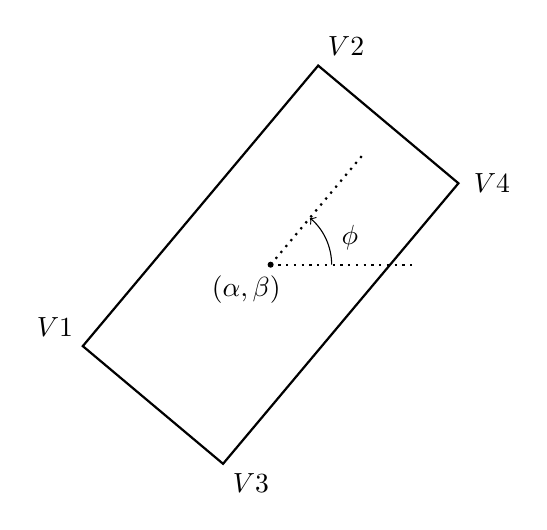
\begin{tikzpicture}[scale=1.55]

% Parameters (arbitrary for illustration)
\def\ll{3}
\def\ww{1.5}
\def\alphaa{-0.5}
\def\betaa{-0.5}
\def\phii{50}

% Derived quantities
\pgfmathsetmacro{\phirad}{\phii * pi / 180}
\pgfmathsetmacro{\hll}{\ll/2}
\pgfmathsetmacro{\hww}{\ww/2}
\pgfmathsetmacro{\ux}{cos(\phii)}
\pgfmathsetmacro{\uy}{sin(\phii)}
\pgfmathsetmacro{\vx}{-sin(\phii)}
\pgfmathsetmacro{\vy}{cos(\phii)}

% Rectangle vertices
\coordinate (V1) at ({\alphaa - \hll*\ux + \hww*\vx}, {\betaa - \hll*\uy + \hww*\vy});
\coordinate (V2) at ({\alphaa + \hll*\ux + \hww*\vx}, {\betaa + \hll*\uy + \hww*\vy});
\coordinate (V4) at ({\alphaa + \hll*\ux - \hww*\vx}, {\betaa + \hll*\uy - \hww*\vy});
\coordinate (V3) at ({\alphaa - \hll*\ux - \hww*\vx}, {\betaa - \hll*\uy - \hww*\vy});

% Draw rectangle
\draw[thick] (V1) -- (V2) -- (V4) -- (V3) -- cycle;

% Draw the black point
\filldraw[black] (\alphaa,\betaa) circle (0.02);

% Add text label near the point
\node at ({\alphaa - 0.2}, {\betaa - 0.2}) {$(\alpha, \beta)$};

% Reference lines for inclination angle
\draw[thick, dotted] (\alphaa,\betaa) -- ++(1.2,0); % x-axis reference
\draw[thick, dotted] (\alphaa,\betaa) -- ++({1.2*cos(\phii)}, {1.2*sin(\phii)}); % inclined direction

% Inclination angle arc and label (slightly lifted)
\draw[->] (\alphaa,\betaa) ++(0:0.5) arc[start angle=0, end angle=\phii, radius=0.5];
\node at ({\alphaa + 0.65*cos(\phirad/2)}, {\betaa + 0.7*sin(\phirad/2) + 0.22}) {$\phi$};

% Vertex labels
\node[above left]  at (V1) {$V1$};
\node[above right] at (V2) {$V2$};
\node[below right] at (V3) {$V3$};
\node[right=2pt] at (V4) {$V4$};

\end{tikzpicture}
\end{center}
\newline
$V1V2$ or $V3V4$ and $V1V3$ or $V2V4$ are the respective sides that represent the length and the width of the rectangle.
\newline
In order to determine the coordinates of the vertices, we begin with the following step. From the known parameters, we first calculate the midpoint coordinates of both the shorter sides (widths). Let us denote midpoint of $V1V3$ as $M$ and midpoint of $V2V4$ as $N$. By simple trigonometry, we can observe the following - 

$$M_x = \alpha-(l/2)*\cos\phi$$

$$M_y = \beta-(l/2)*\sin\phi$$

$$N_x = \alpha+(l/2)*\cos\phi$$

$$N_y = \beta+(l/2)*\sin\phi$$
\newline
where $A_x$ and $A_y$ are the X and Y coordinates of point $A$. The following diagram shows the location of M and N as well.
\begin{center}
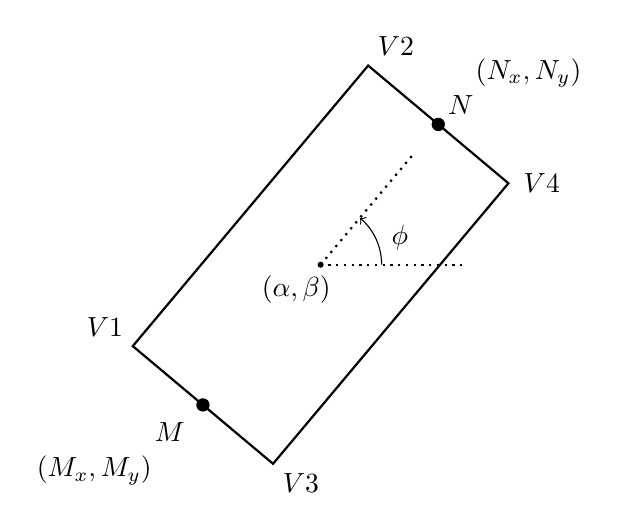
\begin{tikzpicture}[scale=1.55]

% Parameters (arbitrary for illustration)
\def\ll{3}
\def\ww{1.5}
\def\alphaa{-0.5}
\def\betaa{-0.5}
\def\phii{50}

% Derived quantities
\pgfmathsetmacro{\phirad}{\phii * pi / 180}
\pgfmathsetmacro{\hll}{\ll/2}
\pgfmathsetmacro{\hww}{\ww/2}
\pgfmathsetmacro{\ux}{cos(\phii)}
\pgfmathsetmacro{\uy}{sin(\phii)}
\pgfmathsetmacro{\vx}{-sin(\phii)}
\pgfmathsetmacro{\vy}{cos(\phii)}

% Rectangle vertices
\coordinate (V1) at ({\alphaa - \hll*\ux + \hww*\vx}, {\betaa - \hll*\uy + \hww*\vy});
\coordinate (V2) at ({\alphaa + \hll*\ux + \hww*\vx}, {\betaa + \hll*\uy + \hww*\vy});
\coordinate (V4) at ({\alphaa + \hll*\ux - \hww*\vx}, {\betaa + \hll*\uy - \hww*\vy});
\coordinate (V3) at ({\alphaa - \hll*\ux - \hww*\vx}, {\betaa - \hll*\uy - \hww*\vy});

% Draw rectangle
\draw[thick] (V1) -- (V2) -- (V4) -- (V3) -- cycle;

% Draw the black point
\filldraw[black] (\alphaa,\betaa) circle (0.02);

% Add text label near the point
\node at ({\alphaa - 0.2}, {\betaa - 0.2}) {$(\alpha, \beta)$};

% Reference lines for inclination angle
\draw[thick, dotted] (\alphaa,\betaa) -- ++(1.2,0); % x-axis reference
\draw[thick, dotted] (\alphaa,\betaa) -- ++({1.2*cos(\phii)}, {1.2*sin(\phii)}); % inclined direction

% Inclination angle arc and label (slightly lifted)
\draw[->] (\alphaa,\betaa) ++(0:0.5) arc[start angle=0, end angle=\phii, radius=0.5];
\node at ({\alphaa + 0.65*cos(\phirad/2)}, {\betaa + 0.7*sin(\phirad/2) + 0.22}) {$\phi$};
% Vertex labels
\node[above left]  at (V1) {$V1$};
\node[above right] at (V2) {$V2$};
\node[below right] at (V3) {$V3$};
\node[right=2pt] at (V4) {$V4$};

% Midpoints M and N based on given formulas
\pgfmathsetmacro{\Mx}{\alphaa - \hll * \ux}
\pgfmathsetmacro{\My}{\betaa - \hll * \uy}
\pgfmathsetmacro{\Nx}{\alphaa + \hll * \ux}
\pgfmathsetmacro{\Ny}{\betaa + \hll * \uy}

% Plot M and N
\filldraw[black] (\Mx,\My) circle (0.1/2);
\node[below left=3pt] at (\Mx,\My) {$M$};
\node[below left=15pt] at (\Mx,\My) {$(M_x, M_y)$};

\filldraw[black] (\Nx,\Ny) circle (0.1/2);
\node[above right] at (\Nx,\Ny) {$N$};
\node[above right=10pt] at (\Nx,\Ny) {$(N_x, N_y)$};
\end{tikzpicture}
\end{center}
\newline
We can again use simple trigonometry to obtain the coordinates of all the 4 vertices, since we now know the midpoints of the widths.
%\clearpage
The coordinates of the 4 vertices are obtained as follows - 

\[
\begin{aligned}
V1_x &= M_x - \frac{w}{2} \sin\phi, \quad &V1_y &= M_y + \frac{w}{2} \cos\phi \\[6pt]
V2_x &= N_x - \frac{w}{2} \sin\phi, \quad &V2_y &= N_y + \frac{w}{2} \cos\phi \\[6pt]
V3_x &= M_x + \frac{w}{2} \sin\phi, \quad &V3_y &= M_y - \frac{w}{2} \cos\phi \\[6pt]
V4_x &= N_x + \frac{w}{2} \sin\phi, \quad &V4_y &= N_y - \frac{w}{2} \cos\phi
\end{aligned}
\]
\newline
where $A_x$ and $A_y$ are the X and Y coordinates of point $A$.
This is how the obstacle is being defined as a rectangular object. We shall now move on to see how the links of the robot are defined.
\subsection{Defining the First link}
Once we have the obstacle, we can move onto defining the first link of the robot as a simple rod hinged at one end, about the origin of the coordinate system, and having length 3 units. So, the first link can basically describe a circle of radius 3 units, centered at the origin. For computation purposes, we choose the rectangle parameters in such a way that the obstacle is completely or partially inside this circle. The following diagram shows the construction of the first link, and the circle described by it. 


\begin{center}
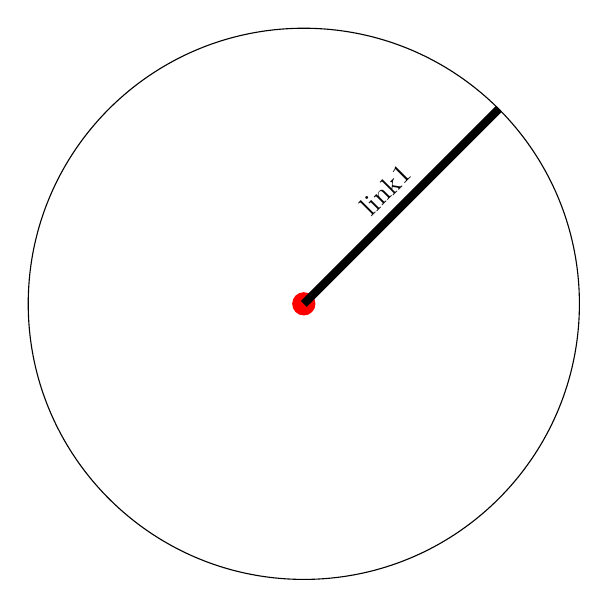
\begin{tikzpicture}
  % Draw circle with radius 3.5
  \draw (0,0) circle (3.5);

  % Draw center dot in red with radius 4pt
  \filldraw[red] (0,0) circle (4pt);

  % Draw radius line with annotation "link1" on the line
  \draw[line width=3pt] (0,0) -- (2.475, 2.475) node[pos=0.5, above, sloped] {link1};

\end{tikzpicture}
\end{center}
We can now place the obstacle fully or partially inside this circle, by choosing appropriate parameters for the rectangle. Note that we shall not place the obstacle in ways that overlap with the origin, because in such cases we cannot construct the first link and it is a collision by default.

\begin{center}
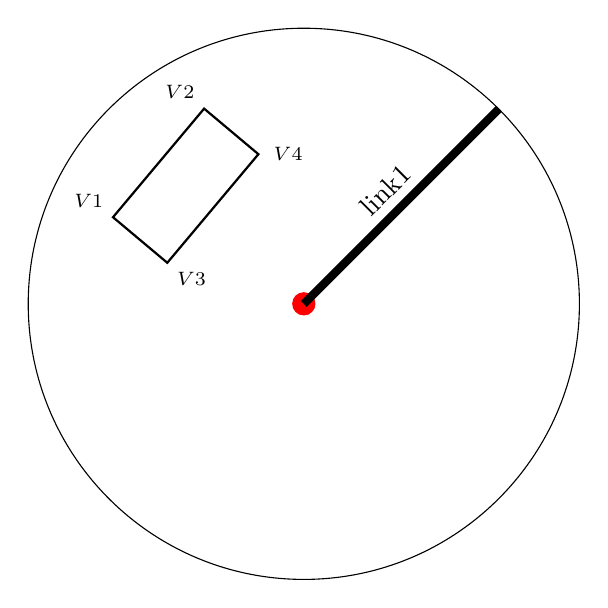
\begin{tikzpicture}
  % Draw circle with radius 3.5
  \draw (0,0) circle (3.5);

  % Draw center dot in red with radius 4pt
  \filldraw[red] (0,0) circle (4pt);

  % Draw radius line with annotation "link1" on the line
  \draw[line width=3pt] (0,0) -- (2.475, 2.475) node[pos=0.5, above, sloped] {link1};

  % Scale and shift obstacle inside circle (more left and up)
  \begin{scope}[scale=0.6, shift={(-2.0,3*1.0)}]  
    % Parameters (arbitrary for illustration)
    \def\ll{3}
    \def\ww{1.5}
    \def\alphaa{-0.5}
    \def\betaa{-0.5}
    \def\phii{50}

    % Derived quantities
    \pgfmathsetmacro{\phirad}{\phii * pi / 180}
    \pgfmathsetmacro{\hll}{\ll/2}
    \pgfmathsetmacro{\hww}{\ww/2}
    \pgfmathsetmacro{\ux}{cos(\phii)}
    \pgfmathsetmacro{\uy}{sin(\phii)}
    \pgfmathsetmacro{\vx}{-sin(\phii)}
    \pgfmathsetmacro{\vy}{cos(\phii)}

    % Rectangle vertices
    \coordinate (V1) at ({\alphaa - \hll*\ux + \hww*\vx}, {\betaa - \hll*\uy + \hww*\vy});
    \coordinate (V2) at ({\alphaa + \hll*\ux + \hww*\vx}, {\betaa + \hll*\uy + \hww*\vy});
    \coordinate (V4) at ({\alphaa + \hll*\ux - \hww*\vx}, {\betaa + \hll*\uy - \hww*\vy});
    \coordinate (V3) at ({\alphaa - \hll*\ux - \hww*\vx}, {\betaa - \hll*\uy - \hww*\vy});

    % Draw rectangle
    \draw[thick] (V1) -- (V2) -- (V4) -- (V3) -- cycle;

    % Draw the black point
    %\filldraw[black] (\alphaa,\betaa) circle (0.02);

    % Add text label near the point
    %\node at ({\alphaa - 0.2}, {\betaa - 0.2}) {$(\alpha, \beta)$};

    % Reference lines for inclination angle
    %\draw[thick, dotted] (\alphaa,\betaa) -- ++(1.2,0); % x-axis reference
    %\draw[thick, dotted] (\alphaa,\betaa) -- ++({1.2*cos(\phii)}, {1.2*sin(\phii)}); % inclined direction

    % Inclination angle arc and label (slightly lifted)
    %\draw[->] (\alphaa,\betaa) ++(0:0.5) arc[start angle=0, end angle=\phii, radius=0.5];
    %\node at ({\alphaa + 0.65*cos(\phirad/2)}, {\betaa + 0.7*sin(\phirad/2) + 0.22}) {$\phi$};

    % Vertex labels with smaller font
    \node[above left]  at (V1) {\scriptsize $V1$};
    \node[above left] at (V2) {\scriptsize $V2$};
    \node[below right] at (V3) {\scriptsize $V3$};
    \node[right=2pt]   at (V4) {\scriptsize $V4$};

  \end{scope}

\end{tikzpicture}
\end{center}
By seeing, we can easily observe that vertices $V_3$ and $V_4$ are the points where the first link will collide when it tries to rotate a full 360 degrees, in both directions. So now we try and come up with an algorithm that gives us the 2 collision points on the rectangle, and essentially the safe operating range of $\theta_1$ (angle rotated by the first link)
\clearpage
\underline{\textbf{Algorithm used to detect the collision limits for link 1:}}
\newline
\newline
There can be 5 broad way of classifying how the obstacle is placed within/near the circle as follows - 
\newline
Case 1: Obstacle is completely inside the circle
\newline
Case 2: Obstacle has just 1 vertex outside the circle
\newline
Case 3: Obstacle has 2 vertices outside the circle
\newline
Case 4: Obstacle has 3 vertices outside the circle
\newline
Case 5: Obstacle has all of its 4 vertices outside the circle
\newline
For the purpose of analysis of the first link, we are not considering obstacles completely outside the circle, nor do we place the obstacle in configurations intersecting the origin, as mentioned before. We can now see the idea that is used to deal with the above 5 cases, and the algorithm that incorporates all the cases.
\newline
\newline
\underline{\textbf{Case 1:}}
\newline
This is the most simplest case, wherein the obstacle completely lies within the circle described by the first link. The obstacle can have any orientation, position and dimensions. So our algorithm must be able to find the collision limits for every feasible configuration satisfying this case. The following diagram shows the collision limits that we are required to determine. We basically have to compute the range of $\theta_1$ for which there will be collision (remaining range is collision-free motion).
\begin{center}
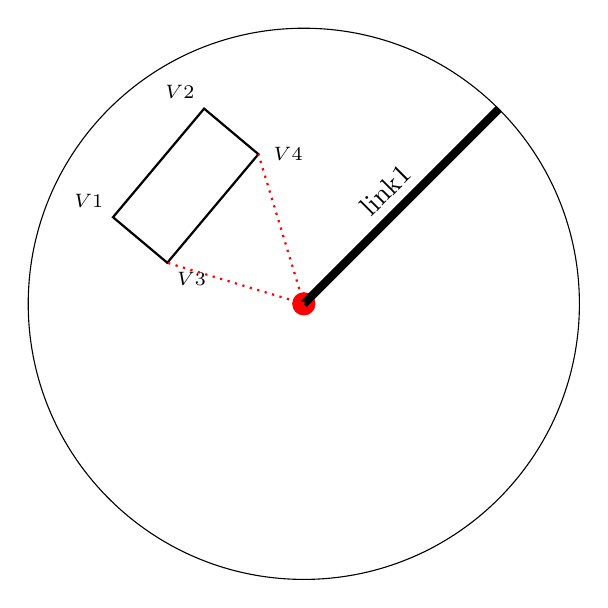
\begin{tikzpicture}
  % Draw circle with radius 3.5
  \draw (0,0) circle (3.5);

  % Draw center dot in red with radius 4pt
  \filldraw[red] (0,0) circle (4pt);

  % Draw radius line with annotation "link1" on the line
  \draw[line width=3pt] (0,0) -- (2.475, 2.475) node[pos=0.5, above, sloped] {link1};

  % --- Scope for obstacle (scaled and shifted)
  \begin{scope}[scale=0.6, shift={(-2.0,3.0)}]  
    \def\ll{3}
    \def\ww{1.5}
    \def\alphaa{-0.5}
    \def\betaa{-0.5}
    \def\phii{50}

    \pgfmathsetmacro{\phirad}{\phii * pi / 180}
    \pgfmathsetmacro{\hll}{\ll/2}
    \pgfmathsetmacro{\hww}{\ww/2}
    \pgfmathsetmacro{\ux}{cos(\phii)}
    \pgfmathsetmacro{\uy}{sin(\phii)}
    \pgfmathsetmacro{\vx}{-sin(\phii)}
    \pgfmathsetmacro{\vy}{cos(\phii)}

    \coordinate (V1) at ({\alphaa - \hll*\ux + \hww*\vx}, {\betaa - \hll*\uy + \hww*\vy});
    \coordinate (V2) at ({\alphaa + \hll*\ux + \hww*\vx}, {\betaa + \hll*\uy + \hww*\vy});
    \coordinate (V4) at ({\alphaa + \hll*\ux - \hww*\vx}, {\betaa + \hll*\uy - \hww*\vy});
    \coordinate (V3) at ({\alphaa - \hll*\ux - \hww*\vx}, {\betaa - \hll*\uy - \hww*\vy});

    % Draw rectangle
    \draw[thick] (V1) -- (V2) -- (V4) -- (V3) -- cycle;

    % Labels
    \node[above left]  at (V1) {\scriptsize $V1$};
    \node[above left]  at (V2) {\scriptsize $V2$};
    \node[below right] at (V3) {\scriptsize $V3$};
    \node[right=2pt]   at (V4) {\scriptsize $V4$};

    % Save transformed V3 and V4 positions globally
    \coordinate (GLOBV3) at (V3);
    \coordinate (GLOBV4) at (V4);
  \end{scope}

  % --- Red dotted radii from origin to V3 and V4 (outside scope!)
  \draw[red, dotted, thick] (0,0) -- (GLOBV3);
  \draw[red, dotted, thick] (0,0) -- (GLOBV4);

\end{tikzpicture}
\end{center}
\clearpage
\underline{\textbf{The Algorithm:}}
\newline
We start off by calculating the angle between the positive X-Axis and the line segment joining the origin and vertex, for each of the 4 vertices.
\newline
Let's say the coordinate of a vertex is ($V_x$, $V_y$), so the corresponding angle between the positive X-Axis and the line segment joining the origin and this vertex is given by the following equation - $$\gamma = \tan^{-1}{(\frac{V_y}{V_x})}$$
\newline
We know that the range of the tan inverse function is from $-\pi$ to $\pi$. Hence we normalize this to $0$ to $2\pi$. So now we know the angles corresponding to all the 4 vertices of the obstacle, lying between 0 and 360 degrees. Let these angles be $\gamma_1, \gamma_2, \gamma_3$, and$ \gamma_4$.
\newline
We now select any 2 of these angles, in all possible combinations. After selecting 2 angles, we compute their absolute difference. Since we have 4 angles, we end up with 6 pair wise differences as follows:
$\gamma_1 - \gamma_2$, $\gamma_1 - \gamma_3$, $\gamma_1 - \gamma_4$, $\gamma_2 - \gamma_3$, $\gamma_2 - \gamma_4$, and 
$\gamma_3 - \gamma_4$.
Whichever difference is maximum, those 2 vertices corresonding to that pair shall give us the collision limits. Note that we only need the absolute value of the difference, so the sign does not matter. In our case, $\gamma_3 - \gamma_4$ turns out to be the maximum of all the 6 pair wise differences. So the vertices $V3$ and $V4$ become the collision limits for link 1.
\newline
\newline
\underline{\textbf{Case 2:}}
\newline
In this case, we have exactly one of the vertices of the obstacle to lie outside the circle. This case turns out be be very similar to the first case. We use the exact same algorithm to find out the collision limits. One thing we do differently here is that we exclude the vertex that lies outside the cirlce. So the pair wise differences are only taken between the remaining 3 vertices which are inside, and that pair is chosen which yields maximum difference. From here, we can get the collision limits for link 1 in the same manner. 
\newline
\newline
In order to determine whether a vertex lies inside or outside the circle, we can simply use the equation of circle to check with the points.
\end{document}

